\documentclass[10pt,a4paper]{amsart}
\usepackage[margin=19mm]{geometry}
\usepackage{amsmath,amssymb,mathtools}
\usepackage[scr=rsfs,cal=euler]{mathalfa}
\usepackage{xfrac}
\usepackage[unicode,hidelinks,bookmarks=false]{hyperref}
\newcommand{\ie}{i.e.\ }
\newcommand{\cf}{cf.\ }
\newcommand{\resp}{respectively\ }
\newcommand{\Subsection}{\subsection}
\providecommand{\nobreakdash}{\nobreak\hbox{-}}
\setlength{\emergencystretch}{2em}
\multlinegap0pt
\usepackage{tikz}
\usepackage[normalem]{ulem}
\usepackage{stackengine}
\usepackage{algorithm}\usepackage{algpseudocode}
\usepackage{float}
\usepackage[shortlabels]{enumitem}
\usepackage{mathtools}
\usepackage{amssymb}
\usepackage{bm}
\newtheorem{lemma}{Lemma}
\newcommand{\E}{\mathcal{E}}
\title{A new family of distances over partially ordered sets}
\author{Astrid A. Olave}
\date{Source: arXiv:2606.06377v1 (CC BY 4.0)}
\begin{document}
\maketitle

\noindent\emph{Source and licence.} A new family of distances over partially ordered sets. Version arXiv:2606.06377v1 (CC BY 4.0), distributed by arXiv under the Creative Commons Attribution 4.0 International licence, http://creativecommons.org/licenses/by/4.0/, as recorded in the arXiv licence metadata for this exact version and shown on the abstract page https://arxiv.org/abs/2606.06377v1. Full licence notice: \texttt{licenses/arxiv-2606.06377-CC-BY-4.0.txt}.\par\smallskip

\noindent\textit{Editorial scope.} Counted unit: the article's lemma lemma:covers\_preserved\_E (source0.tex lines 2288--2291). The article's complete original proof of it is delivered with it (source0.tex lines 2292--2445, one \texttt{proof} environment of 154 lines). No mathematics is written, repaired or re-derived: the statement and the proof are the article's own lines, in the article's own notation, and no retained line is substituted or re-flowed.  Retained uncounted as the source-local context the proof needs: lines 294--297; lines 2232--2235.  Nothing was omitted from any retained span, so the package carries no omission record.  No retained line contains a citation, so the wrapper carries no bibliography and no bibliography entry.  The retained lines contain the article's own diagram code, which the wrapper typesets with the standard tikz packages; no image file is delivered and the package declares no asset dependency.  Editorial formatting only, in addition: an AMS \texttt{amsart} preamble that restates the article's own declarations and macros used by the retained lines, namely the environments \texttt{lemma} on separate counters, together with the standard packages those lines need.  The retained environments print in this document as Lemma 1 in order of appearance, whereas the article prints the same items with the numbering of its own full document.  The complete native source of the article as distributed in the arXiv e-print for this exact version is bundled unchanged as \texttt{sources/202183/source0.tex}.
\begin{lemma}
 Let $P$ and $Q$ be posets equipped with the metric $\mathcal{M}$. If $f$ is a bijection that preserves $\mathcal{M}$ then $f^{-1}$ also preserves $\mathcal{M}$.  
 \label{lemma_f-1_preserves}
\end{lemma}

\begin{lemma}
    Let $f: P \to Q$ a bijection that preserves $\E_1$. If there are $x,y,z \in P$ such that $x \prec z$ and $y \prec z$ and $f(x) \prec f(y)$. Then, the set $\{f(x), f(y), f(z)\}$ together with one or two elements, is a subposet of $Q$ isomorphic to a diamond poset or an up concave pentagon poset respectively.
    \label{lemma:diamond_pentagon_shape}
\end{lemma}

\begin{lemma}
   Let $P$ and $Q$ be posets and let $f: P \to Q$ be a bijection that preserves $\E_1$. If $P$ has elements $x$ and $y$ that are adjacent in $P$ but $f(x)$ and $f(y)$ are not adjacent in $Q$, then $P$ contains a subposet isomorphic to an infinite up diamond–pentagon ladder.
    \label{lemma:covers_preserved_E}
\end{lemma}

\begin{proof}
    Assume that there are $x \prec y$ such that $f(x)$ and $f(y)$ are not adjacent. Given that $\E_1(x,y) = 1$, $f(x)$ and $f(y)$ are not adjacent and $f$ preserves $\E_1$, then there is $z_1 \in Q$ such that  $f(x) \prec z_1$ and $f(y) \prec z_1$. Recall that $f^{-1}$ also preserves $\E_1$ (Lemma \ref{lemma_f-1_preserves}). Hence, by Lemma \ref{lemma:diamond_pentagon_shape}, we obtain that the set 
    $\{x, y, f^{-1}(z_1)\}$ together with one or two elements, is a subposet of $P$ isomorphic to a diamond poset or a concave pentagon poset respectively.  In particular call $w_1 \in P$ the element such that $y = f^{-1}(f(y)) \prec w_1$ and $f^{-1}(z_1) \prec w_1$. Define the  subset $A_1 = \{ x,y,f^{-1}(z_1), w_1 \} \subseteq P$. We use the figure of a trapeze with a left dashed vertical line to represent either a diamond or a up concave pentagon omitting one of the elements

    \begin{center}
    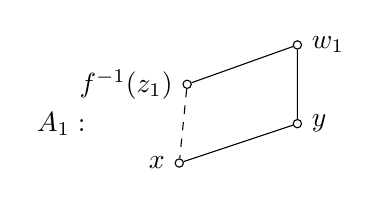
\begin{tikzpicture}[
        node/.style={
        circle, draw=black,
        inner sep=0pt, minimum size=3pt,
        fill=white},
        ]
        \node at (0,0){$A_1:$};
        
        \node (y) [node, label = right: $y$ ]  at (3,0){};
        \node (x) [node, label = left: $x$ ]  at (1.5,-0.5){};
        \node (z1) [node, label = left: $f^{-1}(z_1)$ ]  at (1.6,0.5){};
        \node (w1) [node, label = right: $w_1$]  at (3,1){};
        
        \draw (x) -- (y) (y) -- (w1) (z1) -- (w1);
        \draw [dashed] (z1) -- (x);
    \end{tikzpicture}
    \end{center}
    

    Consider $\hat{x} = y$, $\hat{y} = f^{-1}(z_1)$ and $\hat{z} = w_1$ in $P$. Given that 
    
    \[\hat{x} = y \prec w_1 = \hat{z}, \quad  \hat{y} = f^{-1}(z_1) \prec w_1 = \hat{z} \quad f(\hat{x}) = f(y) \prec z_1 = f(\hat{y}), \] 
    
    by Lemma \ref{lemma:diamond_pentagon_shape} we obtain there is $z_2 \in Q - f(A_1)$ such that $z_1 = f(\hat{y}) \prec z_2$ and $f(w_1) = f(\hat{z}) \prec z_2$. In an analogous way, we find $w_2 \in P - A_1$ with the covering relations $w_1 = f^{-1}(\hat{y}) \prec w_2$ and $f^{-1}(z_2) = f^{-1}(\hat{z}) \prec w_2$ considering in $Q$ the elements 
    \[\hat{x} = z_1, \quad \hat{y} = f(w_1), \quad \hat{z} = z_2, \] 
    again, by Lemma \ref{lemma:diamond_pentagon_shape},  Then, take $A_2 = A_1 \cup \{ f^{-1}(z_2) , w_2) \}$.

    \begin{center}
    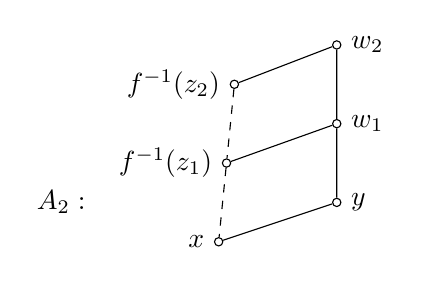
\begin{tikzpicture}[
        node/.style={
        circle, draw=black,
        inner sep=0pt, minimum size=3pt,
        fill=white},
        ]

        \node at (-0.5,0){$A_2:$};
        
        \node (y) [node, label = right: $y$ ]  at (3,0){};
        \node (x) [node, label = left: $x$ ]  at (1.5,-0.5){};
        \node (z1) [node, label = left: $f^{-1}(z_1)$ ]  at (1.6,0.5){};
        \node (w1) [node, label = right: $w_1$]  at (3,1){};
        \node (z2) [node, label = left: $f^{-1}(z_2)$]  at (1.7,1.5){};
        \node (w2) [node, label = right: $w_2$]  at (3,2){};
        
        \draw (x) -- (y) (y) -- (w1) (z1) -- (w1) -- (w2) (z2) -- (w2);
        \draw [dashed] (z2) -- (z1) -- (x);
    \end{tikzpicture}
\hspace{5em}
    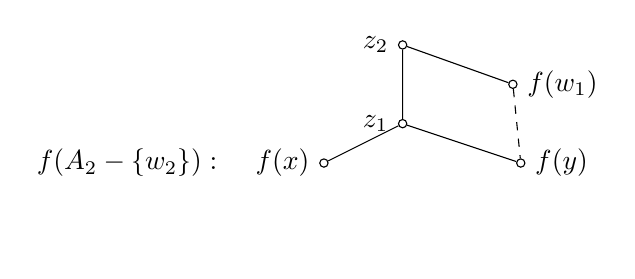
\begin{tikzpicture}[
        node/.style={
        circle, draw=black,
        inner sep=0pt, minimum size=3pt,
        fill=white},
        ]

        \node at (-0.5,0){$f(A_2 - \{w_2\}):$};
        
        \node (y) [node, label = right: $f(y)$ ]  at (4.5,0){};
        \node (x) [node, label = left: $f(x)$ ]  at (2,0){};
        \node (z1) [node, label = left: $z_1$]  at (3,0.5){};
        \node (z2) [node, label = left: $z_2$]  at (3,1.5){};
        \node (w1) [node, label = right: $f(w_1)$]  at (4.4,1){};
        \node at (1,-1){};
        
        \draw (x) -- (z1) (y) -- (z1) -- (z2) (w1) -- (z2);
        \draw [dashed] (w1) -- (y);
    \end{tikzpicture}
    \end{center}

    Recursively, for $n \geq 3$, define $A_n = A_{n-1} \cup \{ f^{-1}(z_n),w_n\}$ where $z_n \in Q - f(A_{n-1})$ is the result of Lemma \ref{lemma:diamond_pentagon_shape} for the elements in $P$
    \begin{equation*}
        \hat{x} = w_{n-2} \quad \hat{y} = f^{-1}(z_{n-1}) \quad \hat{z} = w_{n-1}, 
    \end{equation*}
    
    and $w_n \in P - A_{n-1}$ the result of Lemma \ref{lemma:diamond_pentagon_shape} considering in $Q$,
     \begin{equation*}
        \hat{x} = z_{n-1} \quad \hat{y} = f(w_{n-1}) \quad \hat{z} = z_{n}, 
    \end{equation*}

    \begin{center}
    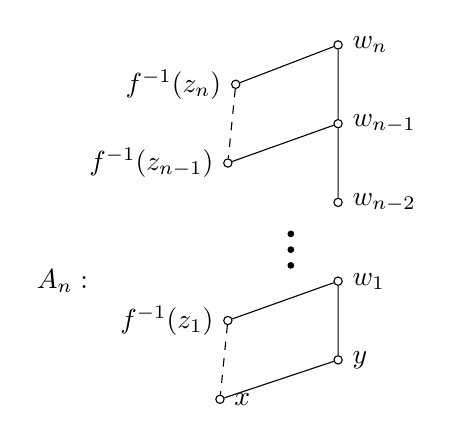
\begin{tikzpicture}[
        node/.style={
        circle, draw=black,
        inner sep=0pt, minimum size=3pt,
        fill=white},
        point/.style={
        circle, draw=black,
        inner sep=0pt, minimum size=2pt,
        fill=black},
        ]

        \node at (-0.5,1){$A_n:$};
        
        \node (y) [node, label = right: $y$ ]  at (3,0){};
        \node (x) [node, label = right: $x$ ]  at (1.5,-0.5){};
        \node (z1) [node, label = left: $f^{-1}(z_1)$ ]  at (1.6,0.5){};
        \node (w1) [node, label = right: $w_1$]  at (3,1){};
        
        
        \node [point] at (2.4,1.2){};
        \node [point] at (2.4,1.4){};
        \node [point] at (2.4,1.6){};

        \node (w) [node, label = right: $w_{n-2}$]  at (3,2){};
        \node (z2) [node, label = left: $f^{-1}(z_{n-1})$]  at (1.6,2.5){};
        \node (w2) [node, label = right: $w_{n-1}$]  at (3,3){};
        \node (z3) [node, label = left: $f^{-1}(z_n)$]  at (1.7,3.5){};
        \node (w3) [node, label = right: $w_n$]  at (3,4){};
        
        \draw (x) -- (y) (y) -- (w1) (z1) -- (w1)  (z2) -- (w2) (z3) -- (w3) (w) -- (w2) -- (w3);
        \draw [dashed] (z3) -- (z2)  (z1) -- (x);
    \end{tikzpicture}
\hspace{5em}
    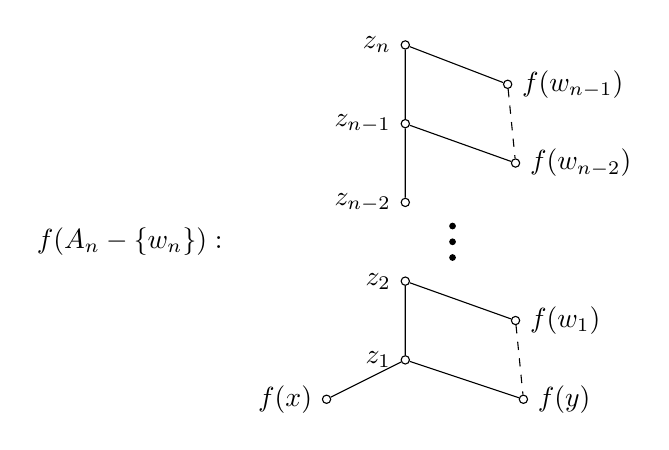
\begin{tikzpicture}[
        node/.style={
        circle, draw=black,
        inner sep=0pt, minimum size=3pt,
        fill=white},
        point/.style={
        circle, draw=black,
        inner sep=0pt, minimum size=2pt,
        fill=black},
        ]

        \node at (-0.5,2){$f(A_n - \{w_n\}):$};

        \node (x) [node, label = left: $f(x)$ ]  at (2,0){};
        \node (y) [node, label = right: $f(y)$ ]  at (4.5,0){};
        \node (z1) [node, label = left: $z_1$]  at (3,0.5){};
        \node (z2) [node, label =  left: $z_2$]  at (3,1.5){};
        \node (w1) [node, label = right: $f(w_1)$]  at (4.4,1){};
        
        \node [point] at (3.6,1.8){};
        \node [point] at (3.6,2){};
        \node [point] at (3.6,2.2){};

        \node (z) [node, label = left: $z_{n-2}$]  at (3,2.5){};
        \node (w2) [node, label = right: $f(w_{n-2})$ ]  at (4.4,3){};
        \node (w3) [node, label = right: $f(w_{n-1})$]  at (4.3,4){};
        \node (z3) [node, label = left: $z_{n-1}$]  at (3,3.5){};
        \node (z4) [node, label =  left: $z_n$]  at (3,4.5){};
        
        \draw (x) -- (z1) (y) -- (z1) -- (z2) (w1) -- (z2) (z) -- (z3) -- (z4) (z3) -- (w2) (z4) -- (w3);
        \draw [dashed] (w3) -- (w2) (w1) -- (y);
    \end{tikzpicture}
    \end{center}

    Let $A = \lim_{n \to \infty} A_n$.  Then $A$ is a subposet of $P$ isomorphic to an infinite up diamond–pentagon ladder.
\end{proof}

\end{document}
